\chapter{Improved Descent Method and Performance Results}
\label{Sec:Numerics}


\section{Introduction} 		\label{Subsec:Numerics-intro}

In this chapter we present an improved version of Algorithm \ref{Alg:PGD} and examine the performance of this improved algorithm.
Section \ref{Subsec:Numerics-improved_PGD} states the improved version of Algorithm \ref{Alg:PGD}, which applies the new termination conditions of Chapter \ref{Sec:PLGD_term_crit} and \textit{the IRAM with adaptive parameter selection} of Chapter \ref{Sec:evol_mats}.
Next, Section \ref{Subsec:Numerics-perf_results} examines the performance of this improved algorithm.
We demonstrate that this improved algorithm is more efficient than Algorithm \ref{Alg:PGD} for a variety of PLGD models with Gaussian noise (\ref{Eqn:PhaseLift-GD_Gaussian_noise}).
We observe that the improved algorithm often reduces the number of matrix-vector products in the EMEP (\ref{Eqn:EMEP_PLGD}) by at least $50\%$ as compared with Algorithm \ref{Alg:PGD}.
Further experiments show that this reduction in the number of matrix-vector products is comparable 
to the reduction observed by solving the \emep \ with the empirically optimal number of requested eigenvalues for each EMEP iterate.
Finally, we demonstrate that the Arnoldi decomposition (\ref{Eqn:Arnoldi_decomp}) size $m = 40$ for the improved algorithm strikes a proper balance between increasing computational efficiency and minimizing data storage.
Note that all experiments in this chapter involve noisy phase retrieval problems and thus we also use the new termination conditions for Algorithm \ref{Alg:PGD} (otherwise Algorithm \ref{Alg:PGD} would not terminate, as discussed in Section \ref{Subsec:PLGD_term_crit-stagnation}).
All experiments in this chapter are available for reproduction.\footnote{\url{https://github.com/Will-Wright/low-rank-opt-rapid-eig}}






\section{Improved Descent Method}	\label{Subsec:Numerics-improved_PGD}


In this section we briefly summarize the contributions of Chapters \ref{Sec:PLGD_term_crit} and \ref{Sec:evol_mats}.  These contributions lead to an improved version of Algorithm \ref{Alg:PGD}.

Section \ref{Subsec:PLGD_term_crit-stagnation} demonstrated that Algorithm \ref{Alg:PGD} fails to converge for PLGD models with Gaussian noise (\ref{Eqn:PhaseLift-GD_Gaussian_noise}).
Section \ref{Subsec:PLGD_term_crit-new_term_crit} then established new termination conditions: the primal difference condition (\ref{Eqn:term_crit_new-primal_difference}) and the dual variable difference condition (\ref{Eqn:term_crit_new-dual_difference}).
Section \ref{Subsec:PLGD_term_crit-new_term_crit} also demonstrated that these new termination conditions accurately identify stagnation of signal recovery progress in Algorithm \ref{Alg:PGD}.
For convenience, we restate these two new termination conditions:
the primal difference condition
\begin{equation}
	\label{Eqn:term_crit_new-primal_difference2}
\frac{| \rho - \hat{\rho} |}{\rho} \leq  \textnormal{tol}_\textnormal{primal} = 10^{-5}, \ \ \rho = ||\caA(xx^*) - b||_2
\end{equation}
and the dual variable difference condition
\begin{equation}
	\label{Eqn:term_crit_new-dual_difference2}
\frac{||y- \hat{y}||_2}{||y||_2} \leq \textnormal{tol}_\textnormal{dual}= 10^{-4},
\end{equation}
where a hat indicates the previous iterate (e.g., $\hat{y} = y_{k-1}$). 


Section \ref{Subsec:evol_mats-adaptive_IRAM} showed that the computational costs of Algorithm \ref{Alg:PGD} are related to the fixed choice of parameters used in the IRAM (Algorithm \ref{Alg:IRAM}), the eigenvalue method used by Algorithm \ref{Alg:PGD}.
Algorithm \ref{Alg:PGD} uses the IRAM with a fixed the number of requested eigenvalues $r = 2$ and Arnoldi decomposition (\ref{Eqn:Arnoldi_decomp}) size $m = 20$.
Section \ref{Subsec:evol_mats-adaptive_IRAM} examined the empirical performance of the IRAM for a range of parameters $r$ to develop \textit{the IRAM with adaptive parameter selection} (Algorithm \ref{Alg:adaptive_IRAM}).
Algorithm \ref{Alg:adaptive_IRAM} increases $m$ to the default value $40$ and adaptively changes $r$ in order to decrease the number of matrix-vector products required by the IRAM.


Applying these the new termination conditions and Algorithm \ref{Alg:adaptive_IRAM} to Algorithm \ref{Alg:PGD}, we have the improved projected gradient descent algorithm for optimizing the PLGD model (\ref{Eqn:PhaseLift-GD_Gaussian_noise}).

\begin{algorithm}[H]
\caption{Improved projected gradient descent method} 	\label{Alg:PGD-improved}

\begin{algorithmic}[1]
	\Statex 	\textbf{Input:} Sensing operator $\caA$ and adjoint $\caA^*$, observation vector $b$,
	initial dual variable $y_0$, 
	estimate of total noise level $\epsilon$,  
	minimum and maximum number of requested eigenvalues, $r_{min}$ and $r_{max}$, 
	Arnoldi decomposition size $m$,
	and convergence tolerances (\ref{Eqn:term_crit_new-primal_difference2}) and (\ref{Eqn:term_crit_new-dual_difference2}).
	\Statex 	\textbf{Output:} Approximate solution signal $x$.
	\Statex		\textbf{Initialization:} Set $T = \{ \emptyset \}$, $R = \{ \emptyset \}$, $k = 0$.
	\While	{conditions (\ref{Eqn:term_crit_new-primal_difference2}) and (\ref{Eqn:term_crit_new-dual_difference2}) are not satisfied}
		\State 		\textit{Compute algebraically largest eigenvalues and corresponding eigenvectors:} 
		Perform Algorithm \ref{Alg:adaptive_IRAM} with inputs $A_k = \caA^*y_k$, $T$, $R$, $r_{min}$, $r_{max}$, and $m$ to obtain	
		$(\lambda_1, v_1)$, $(\lambda_2, v_2)$, $t_k$, $r_k$.
		\State 		\textit{Compute (sub)gradient:} $g = \caA(v_1 v_1^*)$ based on  (\ref{Eqn:GD-subdifferential}).
		\State		Determine differentiability of $\lambda_1(\caA^*y_k)$ based on (\ref{Eqn:GD-diff_tol}).
		\If {$\lambda_1(\caA^*y_k)$ is differentiable}
			\State		\textit{Linesearch:} Perform linesearch (\ref{Eqn:GD-linesearch}) with initial step $\alpha$ (\ref{Eqn:Barzilai-Borwein_steplength}) to obtain $y_{k+1}$.	
		\Else
			\State		\textit{Projected subgradient step:} Set $y_{k+1} = \Pi_\caC (y_k - \alpha g)$ with $\alpha$ from (\ref{Eqn:GD-steplength_sum}).
		\EndIf
		\State		\textit{Primal recovery:} Compute $\hat{x}$ based on (\ref{Eqn:GD-primal_rec2}).
		\State		\textit{Primal refinement:} Find $x_{k+1}$ as the solution to (\ref{Eqn:GD-PFD}) initialized with $\hat{x}$ and $y_{k+1}$.
		\If {$\epsilon = 0$  } {}
			\State		\textit{Dual refinement:} Find $\widehat{y}$ based on (\ref{Eqn:GD-DFP}).
			\State		\textbf{if} $\lambda_1(\caA^* \widehat{y}) < \lambda_1$, set $y_{k+1} = \widehat{y}$.
		\EndIf
			\State	\textit{Update:} Append $t_k$ to $T$, append $r_k$ to $R$, set $k = k+1$.
	\EndWhile
	\State	\textit{Return:} $x = x_k$. 
\end{algorithmic}

\end{algorithm}


For our implementation of Algorithm \ref{Alg:PGD-improved}, we use the default values $r_{min}=2$, $r_{max} = \min\{ 30, m-5 \}$, and $m=40$ (as discussed in Section \ref{Subsec:evol_mats-adaptive_IRAM}).




\section{Performance Results} 		\label{Subsec:Numerics-perf_results}


We now examine the performance behavior of Algorithm \ref{Alg:PGD-improved} for a variety of noisy phase retrieval problems.

First, we compare the performance of Algorithm \ref{Alg:PGD} and Algorithm \ref{Alg:PGD-improved} for a variety of randomly generated and image-based phase retrieval problems.
Figure \ref{Fig:Numerics-ada_vs_orig_various_params} depicts a set of experiments with randomly generated signals.


\begin{figure}[H]
\centering
\hbox{\hspace{-1.1cm} 
	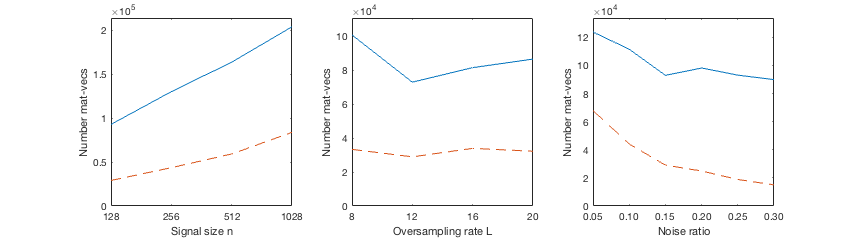
\includegraphics[scale=0.6]{Numerics-ada_vs_orig_various_params}
			}
	\vspace{0.0cm}
	\caption{
	Performance results for PLGD models with Gaussian noise (\ref{Eqn:PhaseLift-GD_Gaussian_noise}), where signals are complex with standard Gaussian distribution (\ref{Def:Gaussian_distribution_complex}).
	Results indicate Algorithm \ref{Alg:PGD} (solid line) and Algorithm \ref{Alg:PGD-improved} (dashed line). 
	Each result is the mean of 10 experiments.
	Left: Varying signal size $n$, with fixed noise ratio $\epsilon_\text{rel} = 0.15$ and oversampling scaled logarithmically with $n$ (i.e., $L = 10, 12, 12, 14$) as indicated in Theorem \ref{Thm:PhaseLift_approx}.
	Middle: Varying oversampling rate $L$, with fixed signal size $n = 128$ and noise ratio $\epsilon_\text{rel} = 0.15$.
	Right: Varying noise ratio $\epsilon_\text{rel}$, with fixed signal size $n = 128$ and oversampling rate $L = 10$.
	}
\label{Fig:Numerics-ada_vs_orig_various_params}
\end{figure}
% experiments.figure.noisyimage_comparison_adaptive_vs_orig

Figure \ref{Fig:Numerics-ada_vs_orig_various_params} demonstrates that Algorithm \ref{Alg:PGD-improved} requires fewer matrix-vector products than Algorithm \ref{Alg:PGD} for a wide range of phase retrieval problems.
The left and middle plots in Figure \ref{Fig:Numerics-ada_vs_orig_various_params} suggest that Algorithm \ref{Alg:PGD-improved} requires about $60\%$ fewer matrix-vector products regardless of signal size $n$ or oversampling rate $L$.
Additionally, the right plot in Figure \ref{Fig:Numerics-ada_vs_orig_various_params} suggests Algorithm \ref{Alg:PGD-improved} may reduce matrix-vector products by $80\%$ or more for problems with significant noise.


We also find that Algorithm \ref{Alg:PGD-improved} is more efficient than Algorithm \ref{Alg:PGD} for image-based phase retrieval problems.
Table \ref{Tab:Numerics-ada_vs_orig_large_images} shows the performance results for two larger images from Figure \ref{Fig:Numerics-large_images}.



\begin{table}[H]
\centering
\begin{tabular}{ |ccc|c|cc|cc| }
 \hline
			&&&  Algorithm \ref{Alg:PGD}
			&  \multicolumn{2}{c|}{Algorithm \ref{Alg:PGD-improved}}
			&	\multicolumn{2}{c|}{Algorithm \ref{Alg:PGD-improved}}	\\
Image & $n$ & $L$ &  	& \multicolumn{2}{c|}{$m=40$}  & \multicolumn{2}{c|}{$m=80$}   \\
 \hline
	\multirow{2}{*}{Figure \ref{Fig:Numerics-large_images}, left} &
   \multirow{2}{*}{$57,600$} &  10 &  562,255  &  297,767 & 47\% &  252,316 & 55\% \\ 
  &&  15 &  647,753  &  301,752 & 53\% &  253,209 & 61\% \\ 
	\multirow{2}{*}{Figure \ref{Fig:Numerics-large_images}, right}  &   
     \multirow{2}{*}{$120,000$} &  10 &  852,633  &  364,164 & 57\% &  287,309 & 66\% \\ 
  &&  15 &  563,085  &  291,630 & 48\% &  256,084 & 55\% \\ 
 \hline
\end{tabular}
\caption{
Performance results for PLGD models with Gaussian noise (\ref{Eqn:PhaseLift-GD_Gaussian_noise}), where signals are the images in Figure \ref{Fig:Numerics-large_images}.
Results indicate total number of matrix-vector products and percent decrease from Algorithm \ref{Alg:PGD}.
Parameter $m$ is the Arnoldi decomposition size (\ref{Eqn:Arnoldi_decomp}) for the IRAM (Algorithm \ref{Alg:IRAM}).
	} 
	\label{Tab:Numerics-ada_vs_orig_large_images}
\end{table}
% experiments.figure.noisyimage_comparison_adaptive_vs_orig



\begin{figure}[H]
\centering
	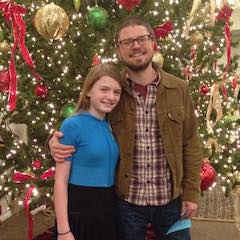
\includegraphics[scale=0.46875]{jul_and_me_orig}
		\hspace{0.1cm}
		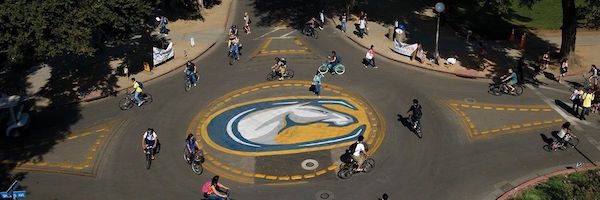
\includegraphics[scale=0.5625]{UCD_orig}
		\vspace{0.3cm} \hspace{0.02cm}
		\\
	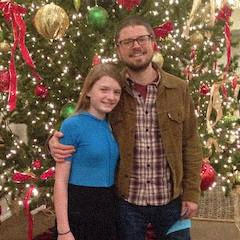
\includegraphics[scale=0.46875]{jul_and_me_L_15_ada40}	
		\hspace{0.1cm}
		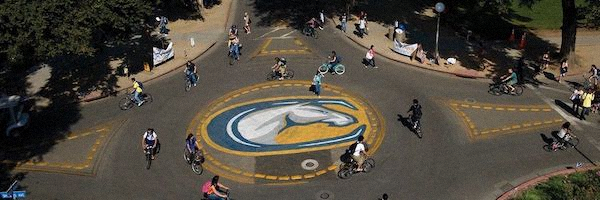
\includegraphics[scale=0.5625]{UCD_L_15_ada40} 
		\vspace{0.0cm}
	\caption{
Images used for experiments in Table \ref{Tab:Numerics-ada_vs_orig_large_images}.
Top left: original image of my daughter and me, image size $240 \times 240 = 57,600$ pixels.
Bottom left: result image after solving EMEP.
Top right: original image of UC Davis roundabout, image size $200 \times 600 = 120,000$ pixels.
Bottom right: result image after solving EMEP.
All experiments have noise ratio $\epsilon_\text{rel} = 0.15$ and oversampling $L = 15$.
	}
\label{Fig:Numerics-large_images}
\end{figure}
% experiments.figure.noisyimage_comparison_adaptive_vs_orig


Table \ref{Tab:Numerics-ada_vs_orig_large_images} demonstrates that the benefits of Algorithm \ref{Alg:PGD-improved} also apply to large-scale phase retrieval problems.
Additionally, a larger Arnoldi decomposition size $m$ further reduces the number of matrix-vector products.
Thus, when solving large-scale problems it may be advisable to consider increasing this parameter beyond the default setting of $m=40$ in Algorithm \ref{Alg:PGD-improved} if memory constraints permit this increase.




Next, we demonstrate that the computational performance improvements of Algorithm \ref{Alg:PGD-improved} are comparable to the improvements of solving the \emep \ with the empirically optimal value $\bar{r}_k$ for each EMEP iterate $k$.
Table \ref{Tab:Numerics-num_matvecs_opt_vs_ada} indicates the number of matrix-vector products for six PLGD models with Gaussian noise (\ref{Eqn:PhaseLift-GD_Gaussian_noise}) using Algorithm \ref{Alg:PGD} ($r=2$), Algorithm \ref{Alg:PGD-improved} ($r$ chosen with Algorithm \ref{Alg:adaptive_IRAM}), and the empirically optimal sequence of values $\bar{r}_k$.



\begin{table}[H]
\centering
\begin{tabular}{ |ccc|c|cc|cc| }
 \hline
			&&&  Algorithm \ref{Alg:PGD}
			&	\multicolumn{2}{c|}{Algorithm \ref{Alg:PGD-improved}  }
			&  \multicolumn{2}{c|}{ Empirically optimal $\bar{r}$ }	\\
$L$ & $\epsilon_\text{rel}$ & EMEP its &  	& \multicolumn{2}{c|}{ $m=40$ }  & \multicolumn{2}{c|}{$m=40$}   \\
 \hline
 5 &  0.05 & 300 &  406,308  &  198,070 & 51\% &  179,807 & 56\%  \\ 
  5 &  0.15 & 300 & 1,099,045  &  258,385 & 76\% &  242,003 & 78\%  \\ 
  5 &  0.30 &  92 &  444,697  &   69,510 & 84\% &   58,780 & 87\%  \\ 
 10 &  0.05 & 153 &   80,453  &   68,709 & 15\% &   61,948 & 23\%  \\ 
 10 &  0.15 & 108 &   88,317  &   57,231 & 35\% &   51,311 & 42\%  \\ 
 10 &  0.30 &  54 &   72,486  &   25,809 & 64\% &   23,217 & 68\%  \\ 
 \hline
\end{tabular}

\caption{
Performance results for PLGD models with Gaussian noise (\ref{Eqn:PhaseLift-GD_Gaussian_noise}) with original signal from Figure \ref{Fig:parrot_signal_iterates} resized to $64 \times 64$ pixels.
Results indicate total number of matrix-vector products and percent decrease from Algorithm \ref{Alg:PGD}.
Parameter $m$ is the Arnoldi decomposition size (\ref{Eqn:Arnoldi_decomp}).
} \label{Tab:Numerics-num_matvecs_opt_vs_ada}
\end{table}
% experiments.figure.noisyimage_adaptive_eig_full_exp


For each of the experiments in Table \ref{Tab:Numerics-num_matvecs_opt_vs_ada}, we see that Algorithm \ref{Alg:PGD-improved} offers nearly the same performance improvement as that of solving the EMEP with the empirically optimal values $\bar{r}_k$.
Notably, experiments in Table \ref{Tab:Numerics-num_matvecs_opt_vs_ada} with a low oversampling rate ($L=5$) shows that Algorithm \ref{Alg:PGD-improved} is particularly effective at decreasing the number of matrix-vector products when there is a large relative difference between the number of matrix-vector products for Algorithm \ref{Alg:PGD} and the empirically optimal choice of values $\bar{r}_k$.
To further explore this performance behavior, Figure \ref{Fig:Numerics-num_eigs_ada_vs_opt} depicts the two PLGD models from Table \ref{Tab:Numerics-num_matvecs_opt_vs_ada} with the largest and smallest relative difference in matrix-vector products (those with $L=5$, $\epsilon_\text{rel} = 0.15$, and $L=10$, $\epsilon_\text{rel} = 0.05$, respectively).




\begin{figure}[H]
\centering
\hbox{\hspace{-1.0cm} 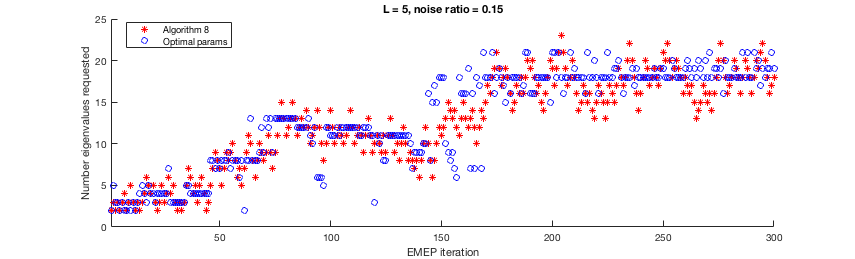
\includegraphics[scale=0.6]{Numerics-num_eigs_ada_vs_opt_1} }\vspace{0.6cm}
\hbox{\hspace{-1.0cm} 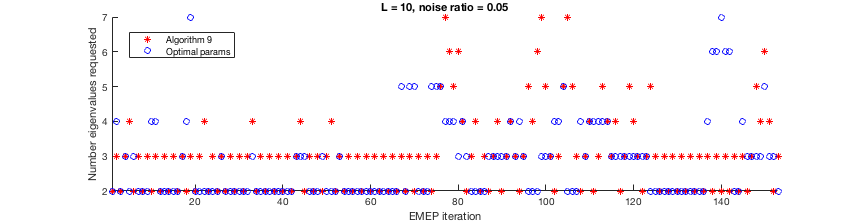
\includegraphics[scale=0.6]{Numerics-num_eigs_ada_vs_opt_2} }
\vspace{0.2cm}
	\caption{
	Number of requested eigenvalues $r$ in the IRAM (Algorithm \ref{Alg:IRAM}) for two PLGD models from Table \ref{Tab:Numerics-num_matvecs_opt_vs_ada}.
	}
\label{Fig:Numerics-num_eigs_ada_vs_opt}
\end{figure}
% experiments.figure.noisyimage_adaptive_eig_full_exp


In both PLGD models depicted in Figure \ref{Fig:Numerics-num_eigs_ada_vs_opt}, the number of requested eigenvalues $r$ selected by Algorithm \ref{Alg:PGD-improved} is usually within 1-3 units from the empirically optimal value $\bar{r}$.
The bottom plot in Figure \ref{Fig:Numerics-num_eigs_ada_vs_opt} suggests that Algorithm \ref{Alg:PGD-improved} required relatively more matrix-vector products than the empirically optimal value $\bar{r}$ because the subroutine Algorithm \ref{Alg:adaptive_IRAM} used in Algorithm \ref{Alg:PGD-improved} always changes the value of $r$ by one or two units, thus shifting away from the optimal value $\bar{r}=2$ for many EMEP iterates.
As we saw in Section \ref{Subsec:evol_mats-adaptive_IRAM} (e.g., Figure \ref{Fig:Numerics-surf_mvs_eig_diffs_2}) the empirically optimal value $\bar{r}$ may shift rapidly for some PLGD models, and thus Algorithm \ref{Alg:adaptive_IRAM} always changes $r$ by one or two units to continue gathering performance information about the EMEP.




Finally, we consider another set of performance results to justify selecting $m=40$ as the default Arnoldi decomposition (\ref{Eqn:Arnoldi_decomp}) size for Algorithm \ref{Alg:PGD-improved}.
Table \ref{Tab:Numerics-num_matvecs_orig_vs_ada} depicts the total number of matrix-vector products required to solve the \emep \ for each PLGD model from Table \ref{Tab:Numerics-num_matvecs_opt_vs_ada} with Algorithm \ref{Alg:PGD-improved} with various parameter values $m$.

\begin{table}[H]
\centering
\begin{tabular}{ |ccc|c|ccccc| }
 \hline
			  \multicolumn{3}{|c|}{n = 4,096} & Algorithm \ref{Alg:PGD}
			&  \multicolumn{5}{c|}{Algorithm \ref{Alg:PGD-improved}}	\\
$L$ & $\epsilon_\text{rel}$ & EMEP its & 	& $m=20$  & $m=40$  & $m=60$  & $m=80$  & $m=100$   \\
 \hline
  5 &  0.05 & 300 &  406,308  &  358,195  &  198,070  &  189,401  &  192,042  &  201,270  \\ 
  5 &  0.15 & 300 & 1,099,045  &  806,412  &  258,385  &  224,048  &  214,118  &  215,392  \\ 
  5 &  0.30 &  92 &  444,697  &  175,669  &   69,510  &   56,193  &   55,146  &   54,987  \\ 
 10 &  0.05 & 153 &   80,453  &   77,768  &   68,709  &   64,300  &   68,602  &   73,754  \\ 
 10 &  0.15 & 108 &   88,317  &   65,833  &   57,231  &   53,261  &   54,388  &   55,308  \\ 
 10 &  0.30 &  54 &   72,486  &   28,799  &   25,809  &   24,699  &   25,113  &   25,491  \\ 
 \hline
\end{tabular}

\caption{
Total number of matrix-vector products for various PLGD models with Gaussian noise	(\ref{Eqn:PhaseLift-GD_Gaussian_noise}) with original signal from Figure \ref{Fig:parrot_signal_iterates} resized to $64 \times 64$ pixels.
Parameter $r$ is the number of requested eigenvalues in the IRAM (Algorithm \ref{Alg:IRAM}) and $m$ is the Arnoldi decomposition (\ref{Eqn:Arnoldi_decomp}) size. 
} \label{Tab:Numerics-num_matvecs_orig_vs_ada}
\end{table}
% experiments.figure.noisyimage_adaptive_eig_full_exp



Table \ref{Tab:Numerics-num_matvecs_orig_vs_ada} demonstrates that Algorithm \ref{Alg:PGD-improved} reduces the number of matrix-vector products from those of Algorithm \ref{Alg:PGD} for all experiments considered.
Yet this cost reduction varies significantly depending on the choice of Arnoldi decomposition (\ref{Eqn:Arnoldi_decomp}) size $m$.
We seek a default setting for the parameter $m$ which is sufficiently large to yield the benefits of Algorithm \ref{Alg:PGD-improved}, yet sufficiently small as not to impact memory constraints.
To select an appropriate default value for $m$, we examine the two experiments from Table \ref{Tab:Numerics-num_matvecs_orig_vs_ada} with $\epsilon_\text{rel} = 0.15, 0.30$ and $L=5$ which have the greatest original number of matrix-vector products, along with the greatest total decrease in cost when using Algorithm \ref{Alg:PGD-improved} with a sufficiently large parameter $m$.
Figure \ref{Fig:Numerics-num_matvecs_ada_for_m_vals} singles out these two experiments, depicting the number of matrix-vector products for each \emep \ iteration.

\begin{figure}[H]
\centering
\hbox{\hspace{-0.9cm} 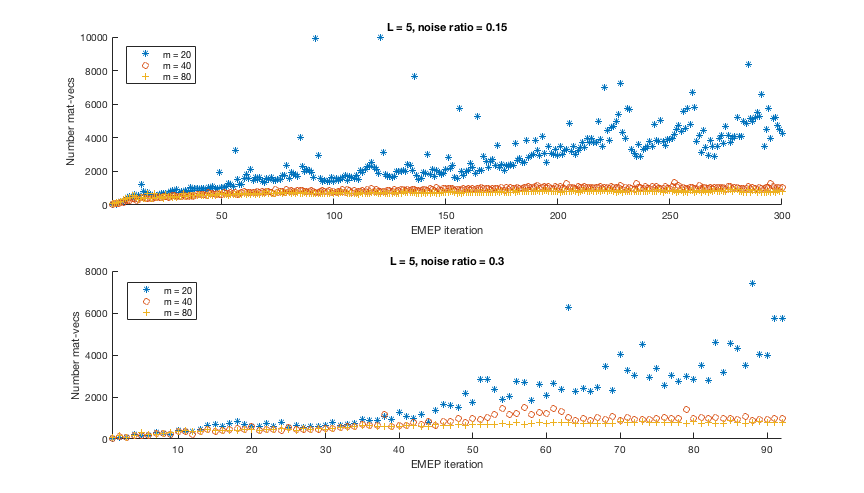
\includegraphics[scale=0.6]{Numerics-num_matvecs_ada_for_m_vals} }\vspace{0.0cm}
	\caption{Number of matrix-vector products for each \emep \ iteration from two experiments in Figure \ref{Fig:Numerics-num_matvecs_ada_for_m_vals} with various Arnoldi decomposition size $m=20, 40, 80$.}
\label{Fig:Numerics-num_matvecs_ada_for_m_vals}
\end{figure}
% experiments.figure.noisyimage_adaptive_eig_full_exp




Figure \ref{Fig:Numerics-num_matvecs_ada_for_m_vals} demonstrates that the Arnoldi decomposition size of $m=20$ is not sufficiently large to allow Algorithm \ref{Alg:PGD-improved} to decrease the number of matrix-vector products.  
The dramatic matrix-vector product spikes for $m=20$ in Figure \ref{Fig:Numerics-num_matvecs_ada_for_m_vals} resemble those first seen in Figure \ref{Fig:EMEP_costs_num_mat_vecs} when using Algorithm \ref{Alg:PGD}.
Yet when the Arnoldi decomposition size is increased to $m=40$, these cost spikes effectively disappear.
The change in number of matrix-vector products between $m=40$ and $m=80$ is minimal for each EMEP iterate.  
Thus the default parameter of $m=40$ for Algorithm \ref{Alg:PGD-improved} strikes the proper balance between efficiency and memory constraints.












